This chapter describes \sys's high-level semantics that a developer can use to
reason about the resulting state of data after a disguise and reveal. Following
this high-level description comes a deeper dive into \sys's API and examples of
how developers can use it.

\section{High-Level Semantics}

\subsection{Disguising and Revealing}
Developers can think about disguising transformations as removing and rewriting
data in the application database.
%
The database starts at some original application state, and alters application
data depending on the disguise specification (\S\ref{s:spec}).  The resulting
state---the disguised data state---is changed only by another disguise, by
revealing the applied disguise, or by normal application updates.
%

%
Disguising already-disguised data can only decrease the amount of information
retained about the original application data state. Removed data cannot be
disguised again. If the original data has been rewritten by prior disguises,
future disguises of the disguised state have access only to the disguised state,
and thus can only further remove aspects of the original data state.
%

%
\sys applies disguises on behalf of either a single user or all users. However,
only a user can reveal a disguise on their data, and must provide a reveal
credential to \texttt{RevealData}.
%

%
Revealing a disguise $D$ on some data disguised by $D$ reverts the changes to
the data applied by $D$ back to the pre-disguised state, except in two cases.
First, if a normal application update has since changed the disguised data, then
the data remains in its updated state and cannot be revealed.
%
Second, if another disguise has since applied changes to the data $D$ disguised,
and that disguise has not yet been revealed, then the data remains in its
current state.
%
Only when all subsequent disguises are revealed does the data revert to the
state prior to $D$.
%
Thus, when multiple disguises apply to the same data, the application data state reflects the
effects of all yet-unrevealed disguises.
%

%
For example, if a post is disguised twice---once to modify the timestamp, and
again to scrub its content---then revealing only one disguise will restore only
that attribute (\eg a timestamp or the post content). 
%
This also applies for disguises that rewrite the same data attributes. For
example, if one disguise decorrelates a post from its author to ``AnonPig''
(\ie by rewriting its \texttt{author} foreign key to the ``AnonPig''
pseudoprincipal) and another disguise decorrelates the post again to
``AnonDog,'' the post will be correlated with ``AnonDog'' even if the
first disguise decorrelating to ``AnonPig'' is revealed.
%
And if the second disguise decorrelating to ``AnonDog'' were revealed
first, the data would remain decorrelated to ``AnonPig'' until the user
also reveals that first decorrelating disguise.
\todo{example figures for both of these.}
%

%
Revealing transformations also apply a developer's provided reveal-time updates
(\S\ref{s:semantics:updates}) to the data to reveal, ensuring that revealed data
reflects global application updates since the time of disguise.
%

\subsection{Disguise Specifications}
\label{s:spec}

%
A developer describes the effects of a disguise (and undone by a
reveal) via disguise specifications.  As previously shown in
Figure~\ref{f:spec}, each specification operation consists of the disguise
operation type, the database table name, 
and a SQL \fn{WHERE} predicate.

%
A disguise is invoked either automatically by the application, or by a specific
user of the application identified by their user ID. 
% 
If disguise is user-specific, then only data that has a foreign key to that
user's identifier (is ``owned'' by that user) and matches the disguise
specification's predicate will be disguised.  Otherwise, the disguise applies to
all data matching the disguise specification's predicate.

This section next dives into the semantics of each disguise operation type.
%

\paragraph{Remove.}
A remove operation removes the entire row that matches the operation's
predicate.
%
Developers should take care to handle referential integrity to removed rows, as
\sys will not cascade-delete referencing rows or introduce placeholders.
(Developers should instead use decorrelate operations to remove principal
rows and replace them with pseudoprincipals).
%

%
A reveal of a remove operation will reinsert all removed rows, unless
reinserting the row will violate a primary key or uniqueness constraint of the
application.
%

%
\paragraph{Modify.}
A modify operation works at per-column granularity, and requires developers to
specify a modification policy for each column to modify in addition to the table
name and predicate.
%
The modification policy informs \sys how to generate new placeholder values for
each column to modify using one of \sys's value generation policies. The current
prototype supports constants (\eg "removed"), random values (\eg a random email
address), and values derived from the prior value (\eg a redacted phone number
with only area code visible).
%

%
Revealing a modify operation restores a row's column back to its state prior
to the disguise \emph{only if} the current column value matches the value
generated by the modify operation during the disguise. This prevents a reveal
from overwriting application changes to the column value since the time of
disguise.
%
Some rows may thus end up partially revealed, with only some modified columns
restored back to the original pre-disguise state.  Developrs can set a (global)
flag to disable partial row reveals, to prevent revealing of any column values
in a row with at least one conflicting column value.
%

%
\paragraph{Decorrelate.}
%
A decorrelate operation requires developers to additionally specify \one{} which
foreign keys for the table rows to rewrite, and \two{} a
\texttt{group\_by} attribute if rows with the same value for that attribute
should refer to the same pseudoprincipal after decorrelation.
%
A decorrelate operation only applies to rows with foreign key relationships to
the principals table (if specified on other foreign keys, the operation will do
nothing).
%
Developers also provide a global pseudoprincipal-generation policy
(using \sys's value generation policies) to tell \sys how to generate per-column
placeholder values.
%

%
If a user invokes the disguise, then \sys only decorrelates the specified
foreign key attributes that refer to that user's identifier, and whose
rows match the predicate. 
%
Otherwise, if the disguise applies over all users, then \sys decorrelates all
specified foreign keys for all rows matching the predicate.
%

%
For all rows to decorrelate with the same \texttt{group\_by} attribute value,
\sys rewrites the foreign keys to decorrelate to the same randomly generated
pseudoprincipal.
%
If no \texttt{group\_by} attribute is specified, each row gets a unique
pseudoprincipal.
%
Thus, no two disguises share the same pseudoprincipals, and no two tables share
the same pseudoprincipals.
%

%
\paragraph{Revealing Decorrelate.}
%
Pseudoprincipals may acquire new references from application objects inserted
after the time of disguise---for example, a decorrelated comment might have new
responses. To ensure that revealing a decorrelate operation---which deletes
pseudoprincipals---preserves referential integrity, developers also inform \sys
how to, during reveal, handle these objects added after disguising that refer
pseudoprincipals of the disguise. 
%
Developers choose between three options for
pseudoprincipal-referring objects: \one{} change the object's reference to point
to the original principal (\texttt{RECORRELATE}); \two{} delete the object
(\texttt{REMOVE}); or \three{} continue referring to the pseudoprincipal
(\texttt{RETAIN}).
%
\todo{figure for each option}

This option is global; another choice of API could support a menu of
options, such as per-table checks and fixes (where the developer specifies
per-table policies) or per-inserted-object ones (where the developer makes
application modifications to log all added references to pseudoprincipals).
%

\subsection{Shared Data.}

%
Many applications support shared data; in Lobsters, for example, messages
between users are owned by both users.
%or co-authored papers in HotCRP.
%
\sys's default semantics for shared data implement an ownership model inspired
by a common treatment of shared data as jointly owned.
%
When a user's disguise removes shared data, \sys decorrelates the data from the \xxing user,
but preserves the data and its association with other owners.
%
\sys removes the data once all users have \xxed it and all ownership links are
to pseudoprincipals.
%
Any owner can reveal the message, which restores the message to the database if
it does not exist, and recorrelates only the revealing user; all disguised
owners remain decorrelated as pseudoprincipals until they also choose to reveal
the message.
%
Regardless of the reveal order, if all owners reveal the message, \sys returns
the message to its original state.
%

%
For each shared data object, each owner has an associated unique
pseudoprincipal. If ony some owners have disguised the row, the row will refer
to the disguised owners' unique pseudoprincipals' identifiers instead of the
owners'.
%
When a user reveals a shared data row, all users still disguised remain 
associated with their unique pseudoprincipal (which can be reused over
multiple remove disguises).
%

\begin{figure}
    \centering
    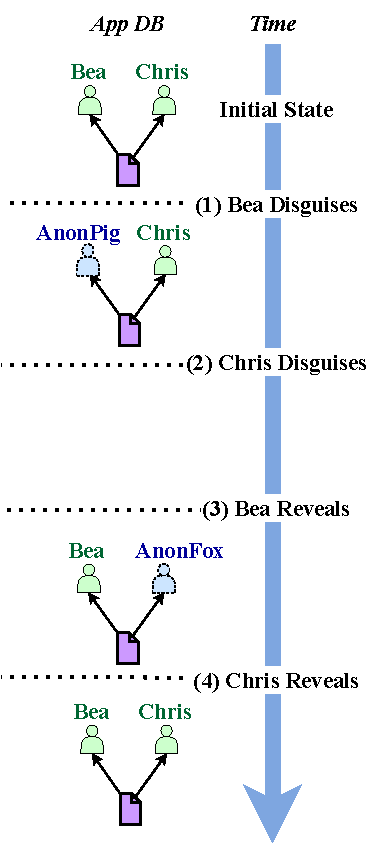
\includegraphics[width=.4\textwidth]{figs/shared_hl}
    \caption[\sys supports joint ownership semantics when disguising shared data.]{\sys supports joint ownership semantics, where shared data is not
    removed until all users have disguised their accounts. Owners can return in
    any order, and the message remains decorrelated from unrevealed owners.}
\label{f:shared:hl}
\end{figure}

%
For instance, consider the scenario in Figure~\ref{f:shared:hl} where Bea and
Chris share a Lobsters message. Bea maps to unique pseudoprincipal AnonPig for this
shared message, and Chris to AnonFox.
\begin{enumerate}[nosep]
    \item[(1)] When Bea \xxs the message, the message is owned by
Chris and a pseudoprincipal;
    \item[(2)] If Chris then \xxs the message, \sys removes it.
    \item[(3)] If Bea reveals the message, this restores the message to the database
and recorrelates only Bea; Chris remains decorrelated as a pseudoprincipal.
\item[(4)] When Chris reveals the message, \sys returns
the message to its original state.
\end{enumerate}
%
\S\ref{s:design:shared} dives deeper in how \sys's design achieves these shared
data semantics.

\subsection{Composition of Disguises.}
Once \sys has decorrelated some user's data to a pseudoprincipal, future
disguises applied by the user will fail to further disguise that
data.
%
If a user wants to further disguise their pseudoprincipal's data,
then the user can grant \sys permission to reveal links to their pseudoprincipal
by providing a reveal credential (their password, private key, or backup token). 
%
\sys will then treat all of the user's pseudoprincipals' data as if they belong
to the user themself, and depending on the disguise specification, will remove,
modify, or create a new pseudoprincipal owner for these pseudoprincipals' data.
%
\S\ref{s:composition} fleshes out \sys's design for disguise composition.

%
%%%%%%%%%%%%%%%%%%%%%%%%%%%%%%%%%%%%%%%%%%%%%%%%%%%%%%%%%%%%%%%%%%%
\section{API Developer Manual}
\label{s:api}

\begin{figure}[t]
\begin{lstlisting}[style=rust,escapeinside={(*}{*)}]
// Generates keypair for p and returns the user's backup credential
(*\textbf{RegisterPrincipal}*)(
        p: UID, 
        pw: Password,
        pubkey: PublicKey, 
        privkey: PrivKey)
    -> RevealCredential;

// disguises principal p according to the spec, 
// optionally over already-disguised data ((*\S\ref{s:composition}*))
(*\textbf{DisguiseData}*)(
        p: Option<UID>, 
        spec: DisguiseSpec,
        principal_gen: PrincipalGenerator,
        schema: Schema,
        disguise_over: Option<RevealCredential>) 
    -> disguiseID;

// Reveals data disguised by s for p with p's password. 
(*\textbf{RevealData}*)(
        p: Option<UID>, 
        did: disguiseID, 
        pp_ref_policy: PseudoprincipalReferencePolicy,
        allow_partial_row_reveal: bool,
        schema: Schema,
        cred: RevealCredential>)
    -> bool;

// Gets principals that p can speak-for.
(*\textbf{CanSpeakFor}*)(p: UID, cred: RevealCredential) -> Vec<UID>;

// Records a reveal-time update spec in the replay log.
(*\textbf{RecordUpdate}*)(update_spec: RevealTimeUpdateSpec) -> bool;
\end{lstlisting}
\caption{\sys's API (Rust-like syntax).}
\label{f:api-high}
\end{figure}
%

Developers add hooks to their application to invoke \sys's API, which consists
of the functions shown in Figure~\ref{f:api-high}. This section describes each
function and how developers would use them to support disguising and revealing.
    

\subsection{\texttt{RegisterPrincipal}}

    Registers an application user as a principal whose data can be disguised and
    revealed. Unique users should not be registered multiple times.  Once
    registered, data of an undeleted user that exists in the database can always
    be disguised and revealed.
    Users deleted by a disguise do not need to reregister if revealed.

    \paragraph{Arguments.} Takes the user's associated unique identifier and unique
    public-private keypair (generated by the user
    client or application).
    %
    The provided public key is used to encrypt the user's disguised data. The
    provided private key and password enable clients to later reveal data using
    either the private key or password.

    \paragraph{Return Value.} 
    The function returns a backup token that the application should return to
    the user client. This token enables the user to reveal in the case they lose
    their password or private key.


\subsection{\texttt{DisguiseData}}
\todo{example effects of disguises---or add examples in
remove/modify/decorrelate sections?}

    Removes or rewrites application data according to the provided disguise
    specification (\ie disguises data). The original data is encrypted and
    stored within the application database; a user must provide credentials to
    invoke with a \texttt{RevealData} call in order to restore the data.
    
    This function may insert pseudoprincipals (anonymous users) into the
    application database if a decorrelation---a rewriting of a foreign key to
    point to an anonymous principal instead of an original principal user---is
    specified by the disguise.  Data disguised within the same disguise and from
    the same table may refer to (via a foreign key) the same pseudoprincipal.
    %
    No two objects from different database tables refer to the same
    pseudoprincipal, and no two disguises' sets of produced pseudoprincipals overlap.

    \paragraph{Arguments.} 
    A disguise is invoked either automatically by the application, or a specific
    user of the application identified by user ID. 
    % 
    If the disguise is invoked on behalf of a specific user, then all predicates
    on specified disguise operations include an "\texttt{AND [fk\_col] = [uid]}"
    clause for all foreign keys to the application's principals table.
    %

    %
    If a user invokes a disguise through the application and provides a reveal
    credential (their password, private key, or backup token), the function will
    disguise data that has already been disguised (\S\ref{s:composition}).
    Depending on the disguise specification, this will remove, modify, or create
    a new pseudoprincipal owner for data with a foreign key to a pseudoprincipal
    instead of the user.
    %

    %
    The developer provides three arguments:
    \begin{itemize}[nosep]
    \item A disguise specification that describes how to disguise data by
    removing, modifying (replacing some or all of its contents with placeholder
    values), or decorrelating, replacing links to users with links to
    pseudoprincipals.
    
    \item A principal generator, which describes how to create a
    pseudoprincipal in the application (global across all disguises).
    
    \item The database schema, which specifies ownership links from data tables to user
    tables via foreign key relationships (global across all disguises).
    \end{itemize}

    \paragraph{Return Value.} 
    The function returns a unique disguise ID for the applied disguise, which
    should be returned to affected users in case they wish to later reveal the
    disguise.

    \paragraph{Shared Data.}
    \todo{repetition?}
    If rows to remove are shared among multiple users, they are only deleted
    from the database once all users have disguised the row. This occurs if
    \one{} all users individually disguise the data, or \two{} the disguise is
    applied over all users (\texttt{p = None}).
   
    If the row is not removed (some owning users have not disguised the row),
    the row will refer to a pseudoprincipal for users who have disguised.

\subsection{\texttt{RevealData}}
\todo{example effects of reveals---or add examples in
remove/modify/decorrelate sections?}


    Restores data disguised by the disguise corresponding to the provided ID to
    the database. Revealing the same disguise ID multiple times will do nothing
    after the first reveal.

    If revealing a row violates database constraints specified in the schema
    (\eg uniqueness, referential integrity, NULl checks), \texttt{RevealData}
    will not restore that row.  \texttt{RevealData} may fail to restore some
    rows, but will still reveal others that successfully pass all constraints
    checks.

    Revealing a row operates on a per-attribute granularity. If an attribute of
    a row at the time of reveal differs from the attribute value set when
    \texttt{DisguiseData} disguised the row, then that attribute of the row will
    not be restored to the original value. This prevents \texttt{RevealData}
    from overwriting an application change since the time of disguise. 
    %
    \texttt{RevealData} will still reveal matching attributes for the row unless
    developers diable partial row removal
    (\texttt{allow\_partial\_row\_reveal}).

    Revealed data will reflect all of the updates registered via
    \texttt{RecordUpdate} since the time of disguise \texttt{did}, applied in
    chronological order.

    \paragraph{Arguments.} 
    A reveal is invoked by a specific
    user of the application identified by user ID. 
    % 
    The user also provides a reveal
    credential (their password, private key, or backup token) and the 
    identifier for the disguise to reveal.

    The developer provides three arguments:
    \begin{itemize}[nosep]
    \item A pseudoprincipal reference policy (\texttt{RECORRELATE}, \texttt{REMOVE},
    or \texttt{RETAIN}) to ensure that reveals of decorrelations preserve
    referential integrity. \texttt{RECORRELATE} ensures that any table rows that
    have been added since the time of disguise, and which have foreign
    key references to a pseudoprincipal row that is removed by the reveal, will
    reference the revealed user replacing the pseudoprincipal.
    \texttt{REMOVE} removes such new references to removed pseudoprincipal rows,
    and \texttt{RETAIN} prevents \texttt{RevealData} from the removing
    pseudoprincipal row and retains any new references to it.
     
    \item A flag specifying whether a row can be partially restored if some
    attributes at the time of reveal differ from the attribute values set when
    disguising the row.

    \item The database schema, which specifies ownership links from data tables to user
    tables via foreign key relationships (global across all disguises).
    \end{itemize}

    \paragraph{Return Value.} 
    Returns true if all rows to reveal pass database constraint checks, and false otherwise.

    \paragraph{Shared Data.}
    \todo{repetition here too?}

\subsection{\texttt{CanSpeakFor}}
\todo{example use of canspeakfor for editing data?}

    Finds all principals in the application identified by user ID that stem from
    a (potentially recursive) decorrelation of user \texttt{p}.
    User \texttt{p} is thus authorized to speak-for any of these principals.

    \paragraph{Arguments.} 
    \texttt{CanSpeakFor} is invoked on behalf of some user with UID \texttt{p},
    and with the user's password.

    \paragraph{Return Value.} 
    A list of all user IDs of principals that \texttt{p} can
    speak-for.

\subsection{\texttt{RecordUpdate}}
\label{s:semantics:updates}
\todo{example use of recordupdate (take from design)}

Enables a developer to perform updates to disguised data prior to revealing it.
Invoking \texttt{RecordUpdate} timestamps and logs a developer-provided update
specification---a data transformation function---to reflect a global update
performed on undisguised data. All updates since the time of disguise will be
performed in chronological order on disguised data prior to revealing it.

If the provided reveal-time update specification relies on data external to the
disguised data to reveal (\eg the current time or state of undisguised data),
\sys cannot ensure correctness when applying the update to disguised data at
reveal time.

    \paragraph{Arguments.} Takes a reveal-time update specification reflecting
    the data transformations performed on table rows. The specification maps a
    set of table rows to a set of updated table rows.

    \paragraph{Return Value.} Returns true on successful recording in \sys's
    log, and false on failure.

\section{\sys Without Encryption}
\label{s:semantics:noencrypt}

Developers may find \sys's threat model unnecessarily strong: perhaps they do
not worry about data breaches, care about regulations like the GDPR, or trust
their application code to not expose disguised data. Instead, these developers
may want to add disuising and revealing without encryption.
%

%
A subset of Edna's API suffices to provide the same semantics for disguises
without encryption. Users do not need to register with \sys; applications can
use normal user authentication to authorize revealing; disguising
already-disguised data no longer requires a user's reveal credential; and
reveal-time updates can be applied immediately to disguised data instead of
logged and applied at reveal time.
%
\S\ref{s:noencrypt} describes how removing encryption changes would
change \sys's design.

%
%Users would provide their application credentials (\eg a username and password)
%to authorize the application to reveal their data.\footnote{While the
%application could reveal data without user permission, this would change the
%semantics of disguise and reveal for a user, causing them to lose control over
%their data's exposure.}
%
%This simplified API still helps address the challenges of maintaining
%referential integrity when a disguise is performed (creating pseudoprincipals as
%placeholder users); composing disguises and reveals in arbitrary orders;
%disguising shared data; and applying global updates to disguised data (albeit
%during update execution, rather than at reveal time).  \S\ref{s:noencrypt}
%describes how removing encryption changes \sys's design.
